\subsection{Research}
\subsubsection{Problem}

Currently, there is no framework available to easily prototype multi-agent UAV systems in a simple environment. Creating a flexible multi-agent architecture would provide an effective solution for developers that want to start prototyping UAV systems. In this project, the architectures of a multi-agent system must be demonstrated with examples. A generic solution must be found for creating easy prototyping. Examples of how to use the different architectures must be present with documentation on how to create them.

In case a company/person wants to develop such technologies, they have to start from scratch which would mean they invest time/money into developing such environments. Using this project, it would erase the issue of a developer having to create their environment. With examples of the architectures already built-in it can boost a project by months.

The current state of the project is a proof of concept with a single UAV, developed for firefighters to give live feedback from the air, scanning the area for possible dangerous chemicals.

\subsubsection{Question}

How can a flexible \acs{mas} architecture for robotics be used in rapid \acs{uav} prototyping?

\subsubsection{Sub-questions}
\begin{enumerate}
    \item What is an Agent?
    \item What is a \acs{mas}?
    \item What is a \acs{mas} architecture?
    \item What is a blackboard communication system?
    \item What are the advantages of a \acs{mas}
    \item What are the necessary/core components of a \acs{mas} architecture?
    \item Are there usable off-the-shelf rapid robot/\acs{uav} prototyping \acs{mas} architectures?
    \item What are the pros and cons of off-the-shelve rapid robot/\acs{uav} prototyping \acs{mas} architectures?
  \end{enumerate}
\newpage

\subsubsubsection{What is an Agent?}

There has yet to be a true definition of what an agent is. A lot of different literatures define an agent in their own way.
All these definitions are strongly based on the background of the research they are conducting. By \citet{AI:agent}, an agent is defined as :

\begin{center}
    \textit{\textbf{"An agent is anything that can be viewed as perceiving its environment through sensors and acting upon that environment through effectors."}}
\end{center}


\begin{figure}[ht]
   \centering
   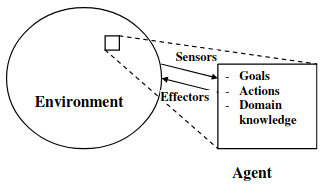
\includegraphics[scale=0.8]{env-agent.png}
   \caption[Agent]{How the environment can be perceived by an agent}
\end{figure}

This means that an agent is an entity that can perceive its environment through sensors and 
perform tasks using data received from these sensors. 

An agent has two basic properties, being autonomous and being situated in an environment \cite{AI:guide}. 
To achieve autonomy the entity must have a goal. An autonomous agent will try and achieve this goal using a set of actions. 
The agent will decide independently what the best set of actions is. During this process there will be no direct intervention from other entities.

To enable an agent to be situated it must have the ability to adapt to dynamic (changing rapidly, unpredictable (not static) 
and unreliable environments (it is not able to predict future states of the environment).

An intelligent agent has additional properties :

\begin{itemize}
   \item Reactive
   \item Proactive
   \item Flexible
   \item Robust
   \item Social
\end{itemize}

A dynamic environment is a repidly changing environment. An agent is often situated in a dynamic environment.
Because of this it will need to adapt to each change to keep pursuing the goal, the agent is reactive. 

The second additional property, proactive, is that the agent will keep pursuing the goal over time. 
If an attempt fails, the agent will need to recover and be robust. 
To achieve robustness the agent will need a range of actions to achieve 
the goal, so it can be flexible in case some actions are not available, have failed before. 

Lastly, an intelligent agent is able to interact with other agents and share its knowledge, the agent is social.
\newpage

\subsubsubsection{What is a \acs{mas}?}

Like the definition of an agent, there has yet to be a true definition for a multi-agent system. 
Yet again there are a lot of definitions, each depending on the background of the research they are conducting.
 For this research the definition is chosen from P. Stone. By \citet{mas:def}, a multi-agent is defined as:

\begin{center}
    \textit{\textbf{"A multi-agent system is a loosely coupled network of problem-solving entities (agents) that work together to find answers to problems that are beyond the individual capabilities or knowledge of each entity (agent)."}}
\end{center}

 
Per definition a multi-agent system is a group of agents organized to solve a problem a single agent would not be able to solve on its own. 
The agents are organized, they have a structure and are able to communicate with each other to share knowledge. 

An agent in a multi-agent system has some important characteristics. As mentioned before, the agent must be autonomous in some form. 
It can make decisions on its own without any intervention. Secondly, no agent has a full view of the world. And thirdly the system must be decentralized. 
There is no controller controlling each agent independently. 

There can be different types of internal hierarchies in a multi-agent system, depending on how the developer wants the agents to work together.

\newpage

\subsubsubsection{What is a \acs{mas} architecture?}

In multi-agent systems there are different ways the agents can be organized. 
Depending on the architecture of this organization the system will adapt to 
the given problem in different ways depending on the architecture. 

When agents work in teams, each team has its function. When a team reaches a goal, it will share this information with the other teams.
\begin{figure}[ht]
    \centering
    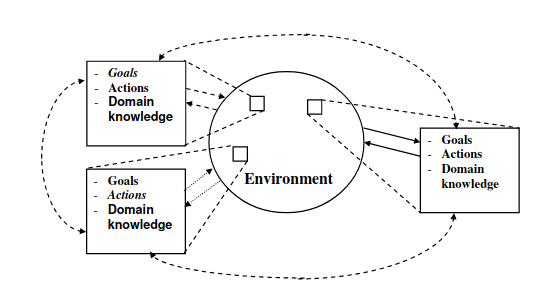
\includegraphics[scale=0.6]{teamcommunication.png}
    \caption[Communication as teams]{Communication as teams\footnotemark.}
\end{figure}

For example a patrol, search, and track problem. Where each team has its own goal. 
Team A will patrol an area and report if it finds some abnormalities. Team B will search for these abnormalities in the area and report any findings to team C. 
Team C will then on its turn start and track these objects.

Coalitions, like teams, consist of multiple UAVS working together. In coalitions not each UAV has the same goal. 
The agents will adapt to the information and the environment to change their goal.

\newpage

\begin{figure}[ht]
    \centering
    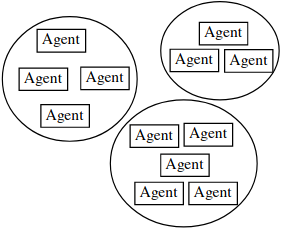
\includegraphics[scale=0.6]{coalitions.png}
    \caption[Communication as coalitions]{Communication as coalitions\footnotemark.}
\end{figure}
Let’s take the same example from teams. Each coalition will take on a subarea of the original area. Within the coalition, 
each agent will take action depending on the current state of the area ( if an object is found or not ). 
Depending on the information an agent can decide to switch actions, for example from searching to tracking.

In a hologenic hierarchy all the agents will communicate with each other, prioritizing the one closest to them. 
Each UAV will share its current state and other agents will adapt to this information. When receiving new information 
from the blackboard system, agent states can change, updating the entire hierarchy. 

\begin{figure}[ht]
    \centering
    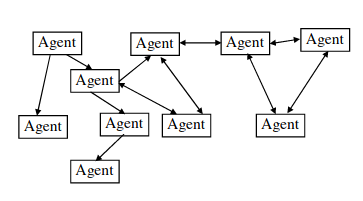
\includegraphics[scale=0.6]{agentComsClosest.png}
    \caption[Communication as hologenic hierarchy]{Communication as hologenic hierarchy\footnotemark.}
\end{figure}
\newpage

\subsubsubsection{What is a blackboard communication system?}

To enable the agents to communicate with each either in a multi-agent system a blackboard communication system is introduced. 
The blackboard system is essentially a node containing all the information for agents to share with each other. 
The information can be separated using different topics depending on the internal hierarchy of the multi-agent system. 
As doing so the agents can be split into groups and only specific information will be shared while still maintaining information sharing inside the groups.

\begin{figure}[ht]
    \centering
    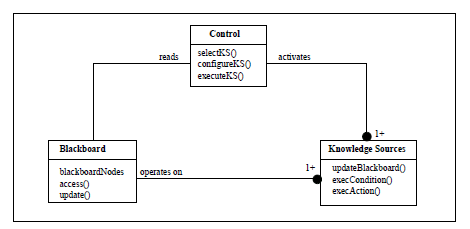
\includegraphics[scale=1.0]{blackboard.png}
    \caption[Blackboard communication]{Blackboard communication}
\end{figure}

\newpage

\subsubsubsection{What are the advantages of a \acs{mas}}

When handling a large problem multi-agent systems provide a robust and scalable solution. 
By spreading the computational workload the system is not only fast but also very reliable.

When an agent fails in a multi-agent system the system will have the availability to 
recover fairly easily from this due to the robustness. 
Control and responsibilities are shared over all the agents. 
The system can tolerate failures of one or more agents by adding the failed actions 
that were being performed by these agents back into the blackboard system. 
Other agents can then try and complete these actions again.

Another advantage of a multi-agent system is scalability. 
Adding another agent to a multi-agent system is easier than expanding an already existing application. 
In a multi-agent system, all the agents are identical therefore introducing a new agent will only update the internal hierarchy.


\subsubsubsection{What are the necessary/core components of a \acs{mas} architecture?}

A multi-system does not have a lot of necessary core components to be able to work. First
of all the system does need to have multiple intelligent agents. These agents need to be
able to ”see” their environment with sensors. These sensors can vary depending on the
system.

The data from the sensors from each agent, the knowledge each agent has, needs to be
sharable with the other intelligent agents. Using this knowledge the system must distribute
the computational load over the agents, No agent is designated as controlling.
\newpage

\subsubsubsection{Are there usable off-the-shelf rapid robot/UAV prototyping \acs{mas} architectures?}

\begin{enumerate}
    \item micros\_mars\_task\_alloc

    \acs{ros} has a package, micros\_mars\_task\_alloc, that is used for multi-task allocation. It is based on
    a multi-agent theory using an ALLIANCE model. The ALLIANCE model uses a cooperative robot team where
    each robot is an intelligent agent.
    
    The ALLIANCE model is based on Brooks' subsumption model. A subsumption architecture is a reactive robot architecture that tries to solve 
    the problem of intelligence from a different perspective than traditional AI \cite{ros:micros_mars_task_alloc}. 
    
    \begin{figure}[ht]
        \centering
        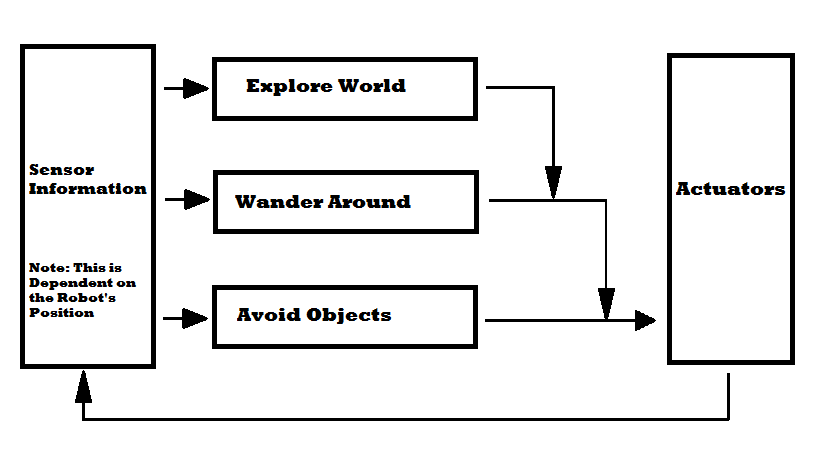
\includegraphics[scale=0.5]{Subsumption_Architecture_Abstract_Diagram.png}
        \caption[Subsumption architecture abstract diagram]{Subsumption architecture abstract diagram\footnotemark.}
    \end{figure}
    
    The ALLIANCE model adds several different behavior sets and behavior layers. These sets and layers are both implemented by following 
    the subsumption model.

    \newpage
    \item FIPA 

    \begin{figure}[ht]
        \centering
        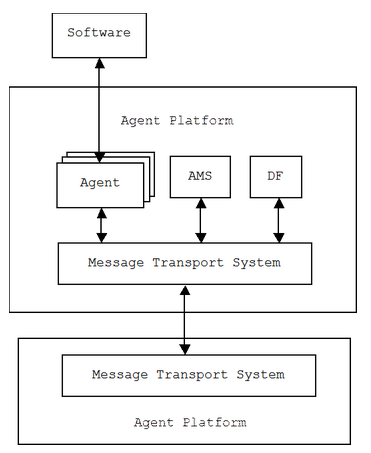
\includegraphics[scale=0.5]{FIPA.png}
        \caption[FIPA]{FIPA diagram\footnotemark.}
    \end{figure}

    \acs{fipa} (Foundation for Intelligent Physical Agents) is an open source agent platform from Nortel Networks. The platform uses an 
    agent communication language that conforms to the \acs{fipa} agent standards. \cite{FIPA-OS}

\end{enumerate}
\newpage

\subsubsubsection{What are the pros and cons of off-the-shelve rapid robot/UAV prototyping \acs{mas} architectures?}

One of the biggest cons with off-the-shelve multi-agent architectures is that they are almost
always designed for a specific research topic. The interactions with the environments are
not generic and prototyping is very difficult because of the limitations in setting the goals
of the intelligent agents. The data sharing between agents is often immutable and therefore
adding sharable knowledge is impossible.

An advantage of using an existing architecture is that the research is already conducted
and the limitations found by the developer. Knowing the limits of an architecture can help
optimize problem-solving by knowing its optimal performance setup.
\newpage

\subsubsection{Research method}
\subsubsubsection{Experiments}

In this project, a lot of different small components work together to form
a bigger system. To test each different component small experiments were tested on a 
smaller scale. Each experiment was run in a smaller system to isolate problems. By isolating a component
it is easier to write generic code for further use.

This provides more insight into each component and how they work. If experiments turn out positive, 
they are implemented in the bigger system.

\subsubsubsection{Observing other projects}

A lot of components already have been coded in other projects in different ways. Observing
other projects gave a lot of insight on how to tackle a problem or on how to evaluate an experiment. 






\newpage